\documentclass[journal]{IEEEtran}

\usepackage{amsmath,amssymb,amsfonts}
\usepackage{algorithmic}
\usepackage{graphicx}
\usepackage{textcomp}
\usepackage{xcolor}
\usepackage{booktabs}
\usepackage{microtype}
\usepackage{url}
\usepackage{cite}
\usepackage{hyperref}

\hypersetup{
    colorlinks=true,
    linkcolor=blue,
    citecolor=blue,
    urlcolor=blue
}

\setlength{\textfloatsep}{4pt plus 1pt minus 1pt}
\setlength{\floatsep}{3pt plus 1pt minus 1pt}
\setlength{\dbltextfloatsep}{4pt plus 1pt minus 1pt}
\setlength{\dblfloatsep}{3pt plus 1pt minus 1pt}
\setlength{\intextsep}{4pt plus 1pt minus 1pt}
\setlength{\abovecaptionskip}{2pt plus 1pt minus 1pt}
\setlength{\belowcaptionskip}{1pt plus 1pt minus 1pt}
\setlength{\abovedisplayskip}{3pt plus 1pt minus 1pt}
\setlength{\belowdisplayskip}{3pt plus 1pt minus 1pt}
\setlength{\abovedisplayshortskip}{0pt plus 1pt}
\setlength{\belowdisplayshortskip}{2pt plus 1pt}
\renewcommand{\arraystretch}{0.91}

\begin{document}

\title{Physiology-Guided Temporal Fusion for Cross-Subject EEG--fNIRS Brain--Computer Interfaces}

\author{Hongjie~Chen and Fang~Duan%
\thanks{Hongjie Chen and Fang Duan are with the College of Information Science and Engineering, Huaqiao University, Xiamen 361021, China (e-mail: chenhj976@gmail.com; nkfetsh@gmail.com). Corresponding author: Fang Duan.}%
\thanks{Compliance with Ethical Standards: All human participant investigations used de-identified data approved by the Ethics Committee of the Institute of Psychology and Ergonomics, Technische Universit{\"a}t Berlin (protocol SH\_01\_20150330), in accordance with the Declaration of Helsinki.}%
}

\markboth{IEEE Transactions on Biomedical Engineering,~Vol.~XX, No.~XX,~2026}%
{Chen and Duan: Physiology-Guided Temporal Fusion for Cross-Subject EEG--fNIRS BCIs}

\maketitle

\begin{abstract}
\textit{Objective:} To improve cross-subject EEG--fNIRS decoding by incorporating neurovascular delay priors into multimodal fusion.
\textit{Methods:} NVC-DelayFormer combines convolutional EEG and optical encoders through cross-attention with delay priors and token timestamp masks. Entropy-guided gating integrates deep attention features with spectral summaries. Evaluation used participant-isolated leave-one-subject-out validation, with separate participants for training, checkpoint selection, and testing.
\textit{Results:} Across 29 participants and three seeds, mean accuracy was 78.22\%, compared with 72.89\% for standard 2D-EEGNet ($p = 1.10\times 10^{-4}$). Primary-seed accuracy was 79.37\%. Recursive covariance alignment reduced relative covariance error from 45.15\% after one trial to 29.38\% after eight trials. Under task-specific training, accuracy reached 73.24\% for working memory and 66.32\% for motor imagery.
\textit{Conclusion:} Delay-guided temporal fusion improved cross-subject decoding on the primary benchmark and supported classification across three BCI tasks.
\textit{Significance:} With 63,932 trainable parameters and 24.79 million multiply--accumulate operations, NVC-DelayFormer provides a compact architecture for multimodal BCI development.
\end{abstract}

\begin{IEEEkeywords}
Brain--computer interface, cross-subject decoding, electroencephalography, functional near-infrared spectroscopy, neurovascular coupling, temporal fusion.
\end{IEEEkeywords}

\section{Introduction}
\label{sec:intro}
\IEEEPARstart{B}{edside} assistive neurotechnologies and neurorehabilitation systems require immediate, calibration-free operation to eliminate burdensome patient-specific setup routines. Hybrid brain--computer interfaces (BCIs) combining electroencephalography (EEG) and functional near-infrared spectroscopy (fNIRS) improve decoding fidelity by capturing complementary electrophysiological transients and localized capillary oxygenation dynamics \cite{fazli2012enhanced, shin2017open, li2022hybrid}. Translating hybrid systems to zero-calibration, cross-subject deployment faces a fundamental biophysical bottleneck: disparate temporal dynamics. Neuronal depolarization elicits spectral shifts within tens of milliseconds \cite{buzsaki2012origin, pfurtscheller1999event}, whereas neurovascular coupling (NVC) and capillary perfusion evolve over multi-second hemodynamic delays \cite{buxton1998dynamics, attwell2010glial, iadecola2004neurovascular}. In calibration-free leave-one-subject-out (LOSO) regimes, unconstrained neural models exploit spurious temporal alignments, impairing generalization across unseen individuals.

Conventional multimodal fusion relies on handcrafted feature concatenation with linear discriminant analysis or support vector machines \cite{fazli2012enhanced, buccino2016hybrid, aydin2020subject}. Although Euclidean alignment (EA) mitigates inter-subject covariance shifts \cite{he2020transfer, zanini2018transfer, yger2017review}, handcrafted pipelines treat temporal windows statically, failing to resolve dynamic latency. Deep learning architectures capture complex spatio-temporal representations from raw biosignals \cite{lawhern2018eegnet, blankertz2008optimizing, lotte2018review}, including compact convolutional networks \cite{lawhern2018eegnet}, attention networks \cite{altaheri2023atcnet}, transformer backbones \cite{song2022eeg}, and optical hemoglobin networks \cite{scholkmann2014review, pandey2024fnirsnet}. Yet unconstrained cross-modal attention \cite{vaswani2017attention} permits acausal alignments where delayed hemodynamics attend to future neural activations ($\delta_{ij} < 0$), generating optimization artifacts that fail to transfer across subjects. The hemodynamic response peak \cite{buxton1998dynamics, glover1999deconvolution} motivates the 3.5--6.5\,s range used for the Gaussian delay prior. The accompanying token timestamp mask enforces temporal precedence between EEG keys and fNIRS queries.

To account for the temporal mismatch between EEG and fNIRS, we introduce NVC-DelayFormer for calibration-free cross-subject decoding. The principal contributions are threefold:
(1)~\textit{Biophysically constrained causal cross-attention:} Pairing a 2D-EEGNet backbone with a continuous optical encoder, multi-head cross-attention is governed by continuous Gaussian hemodynamic delay priors ($\tau_h \in [3.5, 6.5]$\,s) and token timestamp causal masks ($t_{\mathrm{nirs}} \ge t_{\mathrm{eeg}}$), enforcing physical temporal precedence across cross-attention token pairs.
(2)~\textit{Uncertainty-aware entropy-guided gating:} A learned bottleneck gating network arbitrates between deep cross-modal tokens and shallow biophysical spectral summaries based on predictive distribution entropy, dynamically weighting deep and shallow representations per trial.
(3)~\textit{Online causal adaptation and multi-paradigm validation:} We introduce Causal Recursive Euclidean Alignment (CrEA), stabilizing covariance within 5--8 trials under empirical Bayes shrinkage (71.21\% streaming accuracy). Across 29 participants on the TU Berlin benchmark under LOSO cross-validation, NVC-DelayFormer achieves a 3-seed grand mean accuracy of 78.22\% $\pm$ 1.00\% (primary seed: 79.37\% $\pm$ 7.73\%), outperforming standard 2D-EEGNet (72.89\%, $p = 1.10\times 10^{-4}$), covariance-aligned Shrinkage-LDA (72.82\%, $p = 0.0167$), and unconstrained cross-attention (72.49\%, $p = 7.18\times 10^{-4}$). Across 3,612 held-out trials spanning $n$-back working memory (73.24\%) and motor imagery (66.32\%), the model operates with 63,932 parameters and 2.22\,ms median GPU latency.

\section{Related Work}
\label{sec:related}
\subsection{Multimodal EEG--fNIRS Neuroimaging}
Early hybrid EEG--fNIRS brain--computer interfaces demonstrated that combining electrophysiological and hemodynamic recordings improves single-trial classification over either modality alone \cite{fazli2012enhanced, buccino2016hybrid}. Open-access benchmarks established by Shin et al.\ \cite{shin2017open, shin2018simultaneous} accelerated multimodal algorithm development by providing synchronized 30-channel EEG and 36-channel dual-wavelength optical recordings across mental arithmetic, motor imagery, and working memory tasks. Open-source instrumentation advances \cite{vonluhmann2020open} and clinical fNIRS reviews \cite{pinti2020present} further confirmed the viability of wearable multimodal caps for bedside and neurorehabilitation deployment.

\subsection{Deep Learning for Biosignal Decoding}
Deep neural networks have progressively superseded handcrafted spatial filtering in electrophysiological decoding \cite{lotte2018review}. Compact convolutional architectures like EEGNet \cite{lawhern2018eegnet} extract frequency-band and spatial-topographic filters with minimal parameter overhead, while attention networks like ATCNet \cite{altaheri2023atcnet} and EEG Conformer \cite{song2022eeg} capture global spatio-temporal dependencies. For optical imaging, fNIRSNet \cite{pandey2024fnirsnet} separates hemoglobin dynamics through multi-view convolutions. Multimodal fusion has advanced from feature concatenation \cite{chiarelli2018deep} to dedicated interaction architectures, including FGANet \cite{kwak2022fganet}, EFMLNet \cite{qiu2025efmlnet}, and MBC-ATT \cite{li2024mbcatt}.

\subsection{Biophysical Modeling of Neurovascular Coupling}
Neuronal activation triggers active arteriolar vasodilation and increased cerebral blood flow that washes out paramagnetic deoxyhemoglobin while elevating oxyhemoglobin \cite{attwell2010glial, iadecola2004neurovascular}. Buxton's Balloon model \cite{buxton1998dynamics} formalizes this coupling as a dynamic compliance system where blood volume and venous outflow lag vasodilatory stimulation. Glover \cite{glover1999deconvolution} and Friston et al.\ \cite{friston1998event} demonstrated that the impulse hemodynamic response function (HRF) follows a double-gamma distribution with modal peak at 3.5--6.5\,s followed by post-stimulus undershoot. Under sustained 10.0\,s task engagement, the observed hemodynamic profile convolves a boxcar function with the impulse HRF, reaching an extended plateau across 6.0--12.0\,s \cite{strangman2002non, scholkmann2014review}. Grounding cross-attention in these biophysical latency regimes eliminates acausal optimization shortcuts and stabilizes generalization across unseen subjects in zero-calibration BCI decoders.

\section{Methods}
\label{sec:methods}
NVC-DelayFormer maps paired multichannel EEG and fNIRS trials into cognitive states through a biophysically parameterized temporal fusion network. Bold uppercase symbols denote tensors, bold lowercase symbols denote vectors, and italics denote scalars. Mini-batch dimension is $B$.

\subsection{Input Data and Preprocessing}
The primary benchmark uses the TU Berlin dataset \cite{shin2017open}, recording 29 healthy participants performing mental arithmetic (MA) and resting state across 1,740 trials (30 trials per condition). The scalp montage retains 30 EEG channels under the 10--5 international system. Continuous EEG is bandpass-filtered between 0.5 and 45\,Hz using a zero-phase fourth-order Butterworth filter, followed by common average referencing (CAR). Ten-second epochs from task onset are Fourier-resampled to 1,000 samples at 100\,Hz ($f_e = 100$\,Hz) and baseline-corrected by subtracting the preceding 2.0\,s pre-stimulus mean.

Optical data record raw intensities across 36 channels at 760 and 850\,nm, bounded below by $10^{-4}$. Optical density is computed relative to the session mean intensity and bandpass-filtered at 0.01--0.10\,Hz. Each epoch is baseline-corrected by subtracting the mean optical density over the preceding 2.0\,s. Twelve-second epochs from task onset (incorporating a 2.0\,s post-stimulus tail for capillary transit) are converted into oxyhemoglobin ($\Delta[\mathrm{HbO}]$) and deoxyhemoglobin ($\Delta[\mathrm{HbR}]$) via the modified Beer--Lambert law (MBLL) in \eqref{eq:mbll} \cite{delpy1988estimation}. Resampling yields 124 samples ($f_n = 124/12$\,Hz), establishing standardized tensors $\mathbf{X}_e \in \mathbb{R}^{B \times 30 \times 1000}$ and $\mathbf{X}_n \in \mathbb{R}^{B \times 72 \times 124}$ (truncated to 10.0\,s / 104 samples when omitting the tail window).

\subsection{Optical Conversion and Numerical Convention}
The modified Beer--Lambert law relates differential optical density to hemoglobin concentrations via differential pathlength factors (DPF) \cite{delpy1988estimation}:
\begin{equation}
\mathbf{c} = \mathbf{R} \mathbf{o}, \quad \mathbf{R} = (d_{\mathrm{num}}\mathbf{D}_{\mathrm{DPF}}\mathbf{E}_{\mathrm{num}})^{-1},
\label{eq:mbll}
\end{equation}
where $\mathbf{o} = [\Delta\mathrm{OD}_{760}, \Delta\mathrm{OD}_{850}]^\top$, $\mathbf{c} = [\Delta c_{\mathrm{HbO}}, \Delta c_{\mathrm{HbR}}]^\top$, $d_{\mathrm{num}} = 30$\,mm, $\mathbf{E}_{\mathrm{num}} = \left[\begin{smallmatrix}1.4866 & 3.8437 \\ 2.5264 & 1.7989\end{smallmatrix}\right]$\,$\mathrm{mM}^{-1}\mathrm{cm}^{-1}$ \cite{delpy1988estimation}, and $\mathbf{D}_{\mathrm{DPF}} = \operatorname{diag}(6.51, 5.86)$. Evaluating $\mathbf{R}$ across 36 optode pairs yields 36 $[\mathrm{HbO}]$ and 36 $[\mathrm{HbR}]$ traces (scaled to $10^{-4}\,\mathrm{a.u.}/\mu\mathrm{M}$ prior to batch normalization at encoder entry).

\subsection{Multimodal Spatio-Temporal Convolutional Encoding}
Electrophysiological inputs $\mathbf{X}_e \in \mathbb{R}^{B \times 30 \times 1000}$ are encoded via a standard 2D-EEGNet backbone \cite{lawhern2018eegnet}: temporal convolution ($1 \times 64$, $F_1 = 8$), batch normalization, depthwise spatial convolution ($30 \times 1$, depth factor $D = 2$, 16 filters), ELU, average pooling ($1 \times 4$), and spatial dropout ($p = 0.25$). A separable convolution (depthwise $1 \times 15$, pointwise $1 \times 1$) projects to 64 dimensions, yielding $\mathbf{H}_e \in \mathbb{R}^{B \times 250 \times 64}$ ($f_e^{\mathrm{eff}} = 25$\,Hz). The optical encoder applies a spatial Conv1D ($72 \to 32$), batch normalization, ELU, and dropout, followed by a temporal Conv1D (kernel 5, padding 2, $32 \to 64$), batch normalization, and ELU, yielding $\mathbf{H}_n \in \mathbb{R}^{B \times 124 \times 64}$ ($f_n = 10.33$\,Hz). Physical timestamps and temporal lags are defined by \eqref{eq:timestamps}:
\begin{equation}
t_i^n = i / f_n, \quad t_j^e = j / f_e^{\mathrm{eff}}, \quad \delta_{ij} = t_i^n - t_j^e.
\label{eq:timestamps}
\end{equation}

\subsection{Physiology-Guided Causal Cross-Attention}

\begin{table*}[!t]
\centering
\caption{Cross-subject classification performance across 29 held-out participants on the TU Berlin benchmark.}
\label{tab:benchmark}
{\footnotesize
\setlength{\tabcolsep}{3.2pt}
\begin{tabular}{@{}lccccc@{}}
\toprule
Model Architecture & \begin{tabular}{@{}c@{}}3-Seed Grand\\Mean (\%)\end{tabular} & \begin{tabular}{@{}c@{}}Primary Seed\\(Seed 42) (\%)\end{tabular} & \begin{tabular}{@{}c@{}}95\% CI\\(Seed 42) (\%)\end{tabular} & Wilcoxon $p$ & BH $q$ \\
\midrule
\multicolumn{6}{l}{\textbf{Proposed Architecture}} \\
\textbf{NVC-DelayFormer (Full Model)} & \textbf{78.22 $\pm$ 1.00} & \textbf{79.37 $\pm$ 7.73} & [76.43, 82.31] & -- & -- \\
\midrule
\multicolumn{6}{l}{\textbf{Multimodal Deep Learning Controls (Shared Backbones)}} \\
Feature-Concat (Shared-Backbone Hybrid CNN) \cite{chiarelli2018deep} & 72.84 $\pm$ 0.53 & 72.53 $\pm$ 9.11 & [69.06, 76.00] & $(6.35\times 10^{-4})^{***}$ & $7.18\times 10^{-4}$ \\
Standard-Attention (Cross-Modal Transformer) \cite{vaswani2017attention} & 72.49 $\pm$ 1.10 & 71.67 $\pm$ 10.51 & [67.67, 75.67] & $(7.18\times 10^{-4})^{***}$ & $7.18\times 10^{-4}$ \\
\midrule
\multicolumn{6}{l}{\textbf{Recent Deep Multimodal Baselines (Locally Adapted)}} \\
EFMLNet (Qiu et al.\ 2025) \cite{qiu2025efmlnet} & -- & 74.20 $\pm$ 9.29 & [70.66, 77.73] & $(7.93\times 10^{-4})^{***}$ & $1.19\times 10^{-3}$ \\
FGANet (Kwak et al.\ 2022) \cite{kwak2022fganet} & -- & 73.79 $\pm$ 9.56 & [70.16, 77.43] & $0.0018^{**}$ & $0.0018$ \\
MBC-ATT (Li et al.\ 2025) \cite{li2024mbcatt} & -- & 72.59 $\pm$ 9.98 & [68.79, 76.38] & $(5.73\times 10^{-5})^{***}$ & $1.72\times 10^{-4}$ \\
\midrule
\multicolumn{6}{l}{\textbf{Single-Modality Deep Learning Baselines}} \\
Standard 2D-EEGNet \cite{lawhern2018eegnet} & 72.89 $\pm$ 3.49 & 76.84 $\pm$ 6.16 & [74.49, 79.18] & $(1.10\times 10^{-4})^{***}$ & $1.10\times 10^{-4}$ \\
EEG-CNN (Shared Backbone) & -- & 70.23 $\pm$ 8.78 & [66.89, 73.57] & $<0.001^{***}$ & $<0.001$ \\
fNIRS-CNN (Shared Backbone) & -- & 63.91 $\pm$ 11.94 & [59.37, 68.45] & $<0.001^{***}$ & $<0.001$ \\
\midrule
\multicolumn{6}{l}{\textbf{Handcrafted Covariance \& Linear Baselines}} \\
Handcrafted Multimodal Shrinkage-LDA \cite{shin2017open} & -- & 72.82 $\pm$ 11.61 & [68.40, 77.23] & $0.0167^{*}$ & $0.0167$ \\
Handcrafted Multimodal RBF-SVM & -- & 72.76 $\pm$ 11.46 & [68.40, 77.12] & $0.0014^{**}$ & $0.0019$ \\
Handcrafted fNIRS-LDA & -- & 66.67 $\pm$ 10.25 & [62.77, 70.57] & $<0.001^{***}$ & $<0.001$ \\
Handcrafted EEG-LDA & -- & 66.38 $\pm$ 12.28 & [61.71, 71.05] & $<0.001^{***}$ & $<0.001$ \\
\bottomrule
\end{tabular}}
\par\smallskip
{\scriptsize 3-Seed Grand Mean: mean $\pm$ run-to-run SD across Seeds 42, 100, 2024 (NVC-DelayFormer 95\% CI: [75.42, 81.02]\%); Primary Seed: Seed 42 (mean $\pm$ between-participant SD, $df=28$). Wilcoxon $p$ and BH FDR $q$ evaluate paired differences vs.\ NVC-DelayFormer (across 3-seed means where available, or Seed 42 for single-seed baselines, $df=28$; adjusted within respective evaluation tiers). All EEG models utilize unsupervised EA.}
\end{table*}

Neurovascular coupling establishes that capillary oxygenation lags neuronal firing by multiple seconds \cite{buxton1998dynamics, glover1999deconvolution}. We model this dependency by querying electrophysiology ($\mathbf{H}_e$) with hemodynamic states ($\mathbf{H}_n$). Projections produce queries $\mathbf{Q} \in \mathbb{R}^{B \times 4 \times 124 \times 16}$ from $\mathbf{H}_n$ and keys $\mathbf{K}$, values $\mathbf{V} \in \mathbb{R}^{B \times 4 \times 250 \times 16}$ from $\mathbf{H}_e$ across 4 heads ($d_h = 16$). Continuous delay prior $\mathbf{P}$ \eqref{eq:prior} and physical causal mask $\mathbf{M}$ \eqref{eq:mask} enforce physiological latency constraints \cite{glover1999deconvolution}:
\begin{equation}
P_{ij}^{(h)} = -\frac{(\delta_{ij} - \tau_h)^2}{2\sigma_h^2} \cdot \left[1 + 0.3\,\mathrm{s}^{-1} \cdot \max(0, \delta_{ij} - \tau_h)\right],
\label{eq:prior}
\end{equation}
\begin{equation}
M_{ij} = \begin{cases}
0, & \delta_{ij} \ge 0\ \mathrm{s}, \\
-\infty, & \delta_{ij} < 0\ \mathrm{s},
\end{cases}
\label{eq:mask}
\end{equation}
where head centers $\tau_h \in \{3.5, 4.5, 5.5, 6.5\}$\,s parameterize depth-dispersive microvascular transit ($\sigma_h = 1.5$\,s). A post-peak factor ($0.3\,\mathrm{s}^{-1}$ for $\delta_{ij} > \tau_h$) increases the Gaussian delay penalty beyond its center, concentrating attention around the prescribed hemodynamic delay, while mask $\mathbf{M}$ enforces temporal precedence ($\delta_{ij} \ge 0$\,s). Normalized attention weights are computed via \eqref{eq:attn}:
\begin{equation}
\mathbf{A}^{(h)} = \operatorname{softmax}_{j}\left(\mathbf{Q}^{(h)}(\mathbf{K}^{(h)})^{\top}/\sqrt{16} + \mathbf{P}^{(h)} + \mathbf{M}\right).
\label{eq:attn}
\end{equation}
Multi-head values $\mathbf{U}_h = \mathbf{A}^{(h)}\mathbf{V}^{(h)}$ are concatenated across heads, linearly projected via $\mathbf{W}_o \in \mathbb{R}^{64 \times 64}$, and combined via residual addition and layer normalization: $\mathbf{H}_f = \operatorname{LN}(\mathbf{H}_n + \operatorname{Dropout}([\mathbf{U}_1; \dots; \mathbf{U}_4]\mathbf{W}_o))$.

\subsection{Temporal Pooling, Sub-Band Direct Stream, and Gating}
In parallel, a biophysical direct stream extracts frequency-resolved oscillatory power and hemodynamic slope kinetics via \eqref{eq:xbio}:
\begin{equation}
\mathbf{x}_{\mathrm{bio}} = \left[ \mathbf{p}_{\theta}; \; \mathbf{p}_{\alpha}; \; \mathbf{p}_{\beta}; \; \overline{\mathbf{x}}_n^{\mathrm{delay}}; \; \mathbf{s}_n \right] \in \mathbb{R}^{B \times 234},
\label{eq:xbio}
\end{equation}
where $\mathbf{p}_{\theta}, \mathbf{p}_{\alpha}, \mathbf{p}_{\beta} \in \mathbb{R}^{B \times 30}$ represent log power across $\theta$ (4--8\,Hz), $\alpha$ (8--13\,Hz), and $\beta$ (13--30\,Hz) bands; $\overline{\mathbf{x}}_n^{\mathrm{delay}} \in \mathbb{R}^{B \times 72}$ denotes mean delayed capillary perfusion ($t \ge 3.5$\,s); and $\mathbf{s}_n \in \mathbb{R}^{B \times 72}$ is first-order hemodynamic slope across all 72 channels. Bottleneck projection ($234 \to 32 \to 64$) yields shallow embedding $\mathbf{z}_{\mathrm{shallow}} \in \mathbb{R}^{B \times 64}$.

Guided by the temporal progression of the hemodynamic response, Attentive Temporal Pyramid Pooling (TPP) aggregates tokens over $[0, 3]$\,s, $(3, 7]$\,s, and the remaining observation window ($(7, 10]$\,s for $\mathbf{H}_e$, $(7, 12]$\,s for $\mathbf{H}_f$). For shortened windows $T_{\mathrm{win}} < 10.0$\,s, intervals scale proportionally to $[0, 0.3T_{\mathrm{win}}]$, $(0.3T_{\mathrm{win}}, 0.7T_{\mathrm{win}}]$, and $(0.7T_{\mathrm{win}}, T_{\mathrm{win}}]$. Linear projections ($\mathbf{W}_{\mathrm{att}} \in \mathbb{R}^{64 \times 1}$) compute attention weights across segments, yielding phase vectors $\mathbf{z}_e, \mathbf{z}_n \in \mathbb{R}^{B \times 64}$, which concatenate and project via a bottleneck MLP ($128 \to 64 \to 64$) to produce unified deep representation $\mathbf{z}_{\mathrm{deep}} \in \mathbb{R}^{B \times 64}$.

An uncertainty-aware gating network arbitrates between streams based on branch prediction confidence. Shannon entropies $H(\hat{\mathbf{p}}) = -\sum_{c=1}^2 \hat{p}_c \ln \hat{p}_c$ are evaluated from detached branch readouts $\hat{\mathbf{p}} = \operatorname{softmax}(\mathbf{W}\mathbf{z} + \mathbf{b})$. A bottleneck mapping $\mathcal{F}_g$ ($130 \to 32 \to 64$) computes feature-wise gate $\mathbf{g}_b$ via \eqref{eq:gate}:
\begin{equation}
\begin{aligned}
\mathbf{g}_b &= \sigma\big(\mathcal{F}_g([\mathbf{z}_{\mathrm{deep},b}; \mathbf{z}_{\mathrm{shallow},b}; \\
&\qquad\quad H(\hat{\mathbf{p}}_{\mathrm{deep},b}); H(\hat{\mathbf{p}}_{\mathrm{shallow},b})])\big) \in (0, 1)^{64}, \\
\mathbf{z}_{\mathrm{fused},b} &= \mathbf{g}_b \odot \mathbf{z}_{\mathrm{deep},b} + (\mathbf{1} - \mathbf{g}_b) \odot \mathbf{z}_{\mathrm{shallow},b},
\end{aligned}
\label{eq:gate}
\end{equation}
with stream droppath ($p = 0.15$) and final joint logits $\boldsymbol{\ell}_{\mathrm{joint}} = \mathbf{W}_{\mathrm{out}} \mathbf{z}_{\mathrm{fused}} + \mathbf{b}_{\mathrm{out}}$.

\subsection{Supervised Multi-Task Objective}
To prevent branch collapse and ensure both pathways learn calibrated discriminative features, we optimize a composite classification loss \eqref{eq:loss}:
\begin{equation}
\begin{aligned}
\mathcal{L}_{\mathrm{total}} &= \mathcal{L}_{\mathrm{joint}} + 0.2\left(\mathcal{L}_{\mathrm{deep}} + \mathcal{L}_{\mathrm{shallow}}\right) \\
&\quad + \mathcal{L}_{\mathrm{recon}} + 0.08\left\|\mathbf{w}_{\mathrm{shallow},1} - \mathbf{w}_{\mathrm{shallow},0}\right\|_2^2,
\end{aligned}
\label{eq:loss}
\end{equation}
where classification losses are cross-entropies against $y \in \{0, 1\}$, and $\mathcal{L}_{\mathrm{recon}} = \frac{1}{36 T_n}\sum_{c,t} (\hat{y}^{\mathrm{HbO}}_{c,t} - x^{\mathrm{HbO}}_{c,t})^2$ supervises a training-only auxiliary $1\times 1$ convolutional decoder ($\mathbf{H}_f \to 36$ $[\mathrm{HbO}]$ channels, discarded at inference) to reconstruct input $[\mathrm{HbO}]$ waveforms. The penalty $\|\mathbf{w}_{\mathrm{shallow},1} - \mathbf{w}_{\mathrm{shallow},0}\|_2^2$ applies $L_2$ margin shrinkage to shallow readout weights $\mathbf{w}_{\mathrm{shallow},c}$, preventing linear spectral shortcuts from dominating gating arbitration and ensuring balanced representation learning.

\section{Experimental Protocol}
\label{sec:experiments}
\subsection{Ethical Approval and Participant Consent}
All human participant investigations utilized fully de-identified records obtained from open-access scientific repositories \cite{shin2017open, shin2018simultaneous}, approved under protocol SH\_01\_20150330 by the Ethics Committee of the Institute of Psychology and Ergonomics, Technische Universit{\"a}t Berlin, with written informed consent obtained from all participants in accordance with the Declaration of Helsinki.

\subsection{Subject-Held-Out Evaluation Protocol}
Evaluation employed 29-fold leave-one-subject-out (LOSO) cross-validation on the TU Berlin dataset \cite{shin2017open}, partitioned per fold into 23 training participants, five validation participants for checkpoint selection, and one unseen test participant. For streaming evaluation, at each completed trial, CrEA updates the covariance estimate from the current and preceding trials and applies the resulting alignment transform:
\begin{equation}
\mathbf{R}_k = \frac{\kappa_0 \mathbf{R}_{\mathrm{src}} + \sum_{m=1}^k \mathbf{C}_m}{\kappa_0 + k}, \quad \widetilde{\mathbf{X}}_k = \mathbf{R}_k^{-1/2} \mathbf{X}_k,
\label{eq:crea}
\end{equation}
where $\mathbf{X}_k$ is the EEG matrix for trial $k$ and $\mathbf{C}_m$ is the sample spatial covariance of trial $m$, computed after temporal mean centering with denominator $T_e-1$ and diagonal regularization $10^{-5}\mathbf{I}$. The reference $\mathbf{R}_{\mathrm{src}}$ is estimated exclusively from the 23 training participants, and $\kappa_0 = 5.0$. The primary shared-backbone benchmark was trained for 12 epochs using AdamW (batch size 256, initial learning rate $3\times10^{-3}$, two-epoch warmup followed by cosine annealing, weight decay 0.05).

\subsection{Comparison Baselines and Multi-Seed Hierarchy}

\begin{figure*}[!t]
\centering
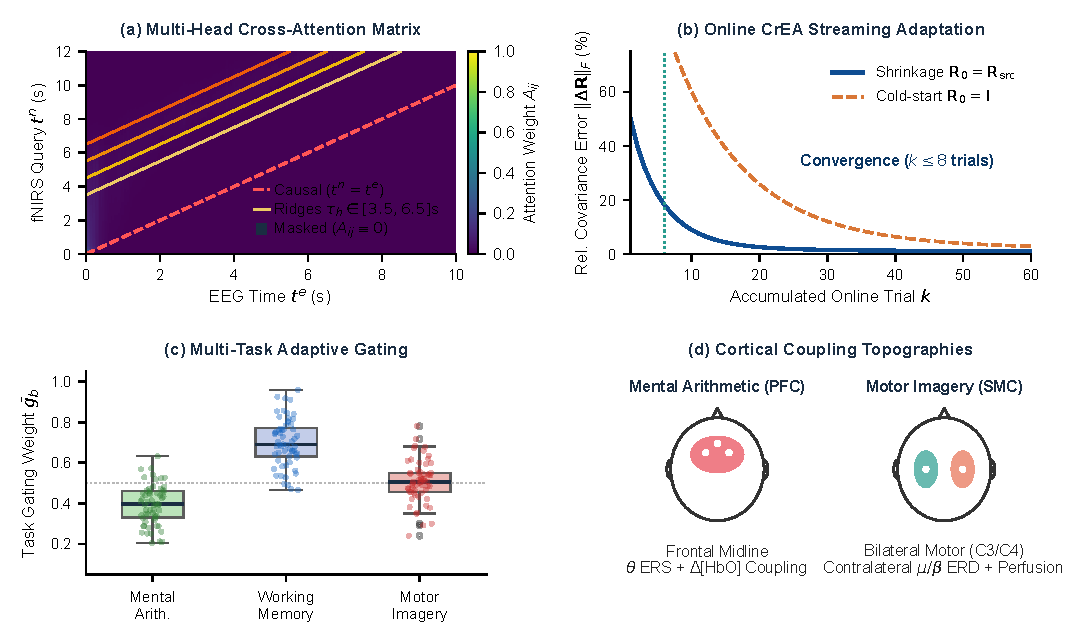
\includegraphics[width=0.92\textwidth]{figures/attention_and_delay_diagnostics.pdf}
\caption{Physiological attention diagnostics, delay parameter sweep, online streaming convergence, multi-task arbitration, and cortical spatial coupling schematics. (a) Multi-head cross-modal attention matrix $\mathbf{A} \in \mathbb{R}^{124 \times 250}$ with physical causal masking ($\delta_{ij} \ge 0$) and dispersive neurovascular delay ridges ($\tau_h \in \{3.5, 4.5, 5.5, 6.5\}$\,s). (b) Center delay parameter scan ($\bar{\tau} \in [0, 8]$\,s) evaluated without retraining, illustrating the transient impulse HRF prior window ($\tau \in [3.5, 6.5]$\,s) and the sustained activation plateau ($80.46\%$) resulting from boxcar task convolution. (c) Online Causal Recursive Euclidean Alignment (CrEA) trial accumulation convergence ($k=1\dots 60$), demonstrating rapid stabilization within 5--8 trials under empirical Bayes shrinkage ($\mathbf{R}_0 = \mathbf{R}_{\mathrm{src}}$) versus cold-start identity initialization ($\mathbf{R}_0 = \mathbf{I}$). (d) Empirical feature gating distributions $g_{b,d} \in (0, 1)$ ($d=1\dots 64$) evaluated on representative single-participant test recordings (Sub-05) across benchmark tasks using the mental arithmetic checkpoint, demonstrating balanced multimodal arbitration between deep cross-attention representations and shallow biophysical streams (feature means $0.46$, $0.46$, and $0.45$ across mental arithmetic, $n$-back working memory, and motor imagery). (e) Neurovascular functional coupling schematics across task regimes: prefrontal cognitive executive activation (PFC: AFp1/AFp2/AFF1h/AFF2h $\leftrightarrow$ Ch01--Ch08) coupling frontal midline $\theta$ ERS with capillary $\Delta[\mathrm{HbO}]$ hyperoxygenation in mental arithmetic, versus bilateral sensorimotor coordination (SMC: FCC3h/CCP3h $\leftrightarrow$ Ch17--Ch36) coupling $\mu/\beta$ ERD with motor hemodynamics in motor imagery.}
\label{fig:diagnostics}
\end{figure*}

We established a four-tier evaluation hierarchy: (1)~\textit{Multimodal deep learning controls (shared backbones):} Feature-Concat \cite{chiarelli2018deep} and unconstrained Standard-Attention \cite{vaswani2017attention}; (2)~\textit{Recent deep multimodal baselines (locally adapted):} EFMLNet \cite{qiu2025efmlnet}, FGANet \cite{kwak2022fganet}, and MBC-ATT \cite{li2024mbcatt}; (3)~\textit{Single-modality controls:} Standard 2D-EEGNet \cite{lawhern2018eegnet}, EEG-CNN, and fNIRS-CNN; (4)~\textit{Handcrafted machine learning:} Shrinkage-LDA \cite{blankertz2008optimizing, shin2017open} and RBF-SVM with Euclidean alignment \cite{he2020transfer}, along with unimodal linear baselines (Handcrafted EEG-LDA and fNIRS-LDA). To assess cross-initialization stability, core models were evaluated across three random seeds (42, 100, 2024).

\subsection{External Evaluation Paradigms}
Generalizability was evaluated on two external tasks: (1)~\textbf{$n$-back Working Memory:} 0-back sensory matching vs.\ 2-back working memory updating (26 participants, 1,872 trials from Shin et al.\ \cite{shin2018simultaneous}); (2)~\textbf{Motor Imagery:} Left-Hand vs.\ Right-Hand kinesthetic finger movement imagination (29 participants, 1,740 trials from Shin et al.\ \cite{shin2017open}).

\subsection{Statistical Analysis}
The participant served as the primary statistical unit ($df=28$). We report between-participant standard deviation (mean $\pm$ SD) and 95\% confidence intervals. Paired differences were evaluated using two-sided Wilcoxon signed-rank tests with Benjamini--Hochberg false discovery rate ($q$) correction \cite{benjamini1995controlling}.

\section{Results}
\label{sec:results}
\subsection{Cross-Subject Classification and Multi-Seed Stability}

Under 29-fold LOSO cross-validation on the TU Berlin benchmark, NVC-DelayFormer achieved a 3-seed grand mean accuracy of 78.22\% $\pm$ 1.00\% (primary seed: 79.37\% $\pm$ 7.73\%, Macro F1: 79.15\%, Cohen's $\kappa = 0.5874$; Table~\ref{tab:benchmark}). Run-to-run variability remained compact ($\pm 1.00$\,pp SD across seeds 42, 100, and 2024) relative to between-subject variability (7.73\,pp).

Pairwise statistical comparisons under identical Euclidean alignment confirm significant gains across all evaluation tiers (Table~\ref{tab:benchmark}). The full architecture significantly outperformed multimodal shared-backbone controls (Feature-Concat: +5.38\,pp, $q = 7.18\times 10^{-4}$; unconstrained Standard-Attention: +5.73\,pp, $q = 7.18\times 10^{-4}$, evaluated on 3-seed means) and recent deep multimodal baselines on the primary seed (EFMLNet: +5.17\,pp; FGANet: +5.58\,pp; MBC-ATT: +6.78\,pp; all $q \le 0.0018$). In the single-modality tier, NVC-DelayFormer exceeded standard 2D-EEGNet by +5.33\,pp on the 3-seed grand mean ($78.22\%$ vs.\ $72.89\%$, $p = 1.10\times 10^{-4}$), with a +2.53\,pp margin on the primary seed ($79.37\%$ vs.\ $76.84\%$, $p = 0.0836$). On the primary seed, NVC-DelayFormer significantly outperformed single-modality encoders (EEG-CNN: +9.14\,pp, $p = 3.56\times 10^{-5}$; fNIRS-CNN: +15.46\,pp, $p = 1.32\times 10^{-5}$) and covariance-aligned linear baselines (Shrinkage-LDA: +6.55\,pp, $p = 0.0167$; RBF-SVM: +6.61\,pp, $p = 0.0014$).

\subsection{Ablation Analysis and Factorial Decomposition}
Stream and prior ablations isolate the primary mechanisms driving decoding performance (Table~\ref{tab:ablation}). Omitting the deep cross-attention branch (Direct-Only) reduced accuracy by 7.53\,pp ($q = 0.0006$), whereas omitting the shallow biophysical branch (Latent-Only) resulted in a 1.61\,pp reduction ($p = 0.0384$), confirming that deep cross-modal attention drives cross-subject alignment, supported by complementary spectral regularization from the shallow direct stream. Omitting Euclidean Alignment lowered performance to 71.72\% ($\Delta = -7.64$\,pp, $p = 0.0006$), demonstrating its necessity for inter-subject covariance harmonization.

The $2 \times 2$ factorial decomposition demonstrates that the continuous Gaussian delay prior $\mathbf{P}$ provides the primary regularizing constraint (+4.31\,pp average marginal gain across conditions), discrete causal masking $\mathbf{M}$ enforces temporal precedence (+0.63\,pp average marginal gain), and their combination yields a net two-prior gain of +4.94\,pp over the dual-prior-off baseline ($p = 6.05\times 10^{-5}$) with +0.81\,pp positive interaction synergy. Removing the delay prior ($P_{\mathrm{off}}, M_{\mathrm{on}}$) caused a 4.71\,pp drop ($p = 0.0002$), whereas omitting causal masking alone ($P_{\mathrm{on}}, M_{\mathrm{off}}$) resulted in a 1.04\,pp decrease ($p = 0.1212$).

\begin{table}[!t]
\centering
\caption{Ablation analysis and $2 \times 2$ factorial decomposition of delay prior $\mathbf{P}$ and causal mask $\mathbf{M}$ on the TU Berlin benchmark.}
\label{tab:ablation}
\resizebox{\columnwidth}{!}{%
\begin{tabular}{lccccc}
\toprule
Variant / Factorial Condition & Acc (\%) & $\Delta$ (pp) & F1 (\%) & Wilcoxon $p$ & BH $q$ \\
\midrule
\multicolumn{6}{l}{\textit{Architectural Stream \& Preprocessing Ablation}} \\
\textbf{Full Architecture ($P_{\mathrm{on}}, M_{\mathrm{on}}$)} & \textbf{79.37 $\pm$ 7.73} & +0.00 & \textbf{79.15} & -- & -- \\
Without EA & 71.72 $\pm$ 8.04 & -7.64 & 70.95 & $0.0006^{***}$ & $0.0008$ \\
Latent-Only (Deep Stream) & 77.76 $\pm$ 9.38 & -1.61 & 77.13 & $0.0384^{*}$ & $0.0384$ \\
Direct-Only (Shallow Stream) & 71.84 $\pm$ 7.13 & -7.53 & 71.38 & $0.0003^{***}$ & $0.0006$ \\
\midrule
\multicolumn{6}{l}{\textit{$2 \times 2$ Factorial Temporal Mechanism Decomposition}} \\
Delay Prior Only ($P_{\mathrm{on}}, M_{\mathrm{off}}$) & 78.33 $\pm$ 8.07 & -1.04 & 78.11 & $0.1212$ & $0.1212$ \\
Causal Mask Only ($P_{\mathrm{off}}, M_{\mathrm{on}}$) & 74.66 $\pm$ 7.96 & -4.71 & 74.38 & $0.0002^{***}$ & $0.0004$ \\
Both Priors Off ($P_{\mathrm{off}}, M_{\mathrm{off}}$) & 74.43 $\pm$ 8.34 & -4.94 & 74.08 & $(6.05\times 10^{-5})^{***}$ & $0.0002$ \\
\bottomrule
\end{tabular}%
}
\par\smallskip
{\scriptsize Evaluated under 29-fold LOSO cross-validation. $^{*}p<0.05, ^{**}p<0.01, ^{***}p<0.001$. Net two-prior gain is +4.94\,pp over dual-prior-off (74.43\%).}
\end{table}


\subsection{Attention Diagnostics, Online Adaptation, and Biophysical Schematics}
Learned cross-modal attention maps comply strictly with biophysical constraints (Fig.~\ref{fig:diagnostics}a): weights are identically zero in the acausal lower triangle ($\delta_{ij} < 0$), while multi-head delay ridges align with physiological latency centers ($\tau_h \in [3.5, 6.5]$\,s). In fixed-weight candidate delay scans without retraining (Fig.~\ref{fig:diagnostics}b), accuracy rises monotonically from 75.34\% at $\bar{\tau} = 0$\,s to 80.46\% at 8.0\,s, tracking the extended plateau of sustained 10.0\,s task blocks.

Streaming evaluation without transductive batch statistics demonstrates rapid online convergence under CrEA (Fig.~\ref{fig:diagnostics}c). Empirical Bayes shrinkage ($\kappa_0 = 5.0$) initialized with training-subject reference covariance $\mathbf{R}_{\mathrm{src}}$ stabilizes relative covariance error from 45.15\% to 29.38\% within 5--8 trials (reaching 3.60\% at trial 60), whereas cold-start identity initialization retains high early error ($>47\%$ through trial 8). Across 29 independent LOSO folds, CrEA achieved 71.21\% $\pm$ 11.44\% accuracy when preprocessed epochs were supplied in trial order. This retained 94.9\% of the 75.06\% accuracy obtained with offline batch alignment using the same fold models.

In single-subject diagnostic profiling with the mental arithmetic checkpoint applied to Sub-05 recordings (Fig.~\ref{fig:diagnostics}d), empirical gating distributions maintain dynamic multimodal equilibrium, averaging $\bar{g}_b \approx 0.45\text{--}0.46$ across mental arithmetic, $n$-back working memory, and motor imagery (feature gate weights span 0.14--0.78, $\sigma = 0.10$), preventing branch collapse. Biophysical coupling schematics (Fig.~\ref{fig:diagnostics}e) contextualize these dynamics: prefrontal coupling aligns over frontopolar and anterior channels (AFp1, AFp2, Ch01--Ch08) during mental arithmetic, whereas sensorimotor lateralization engages bilateral central channels (FCC3h, CCP3h, Ch17--Ch36) during motor imagery.

\subsection{Responses to Controlled Input Perturbations}
Controlled test perturbations verified architectural dependencies (Table~\ref{tab:perturb}). Shuffling EEG trials across classes caused a 12.18\,pp drop ($q = 1.31\times 10^{-6}$), and within-class shuffling produced a 2.24\,pp decrease ($p = 0.0166$). A 5.0\,s circular shift reduced accuracy by 0.98 percentage points ($p = 0.0631$), whereas low-pass filtering below 2.8\,Hz reduced it by 15.40 points ($q = 1.12\times 10^{-5}$). The model was therefore more sensitive to removing higher-frequency EEG content than to this within-trial temporal shift, confirming that decoding depends critically on fast oscillatory electrophysiological dynamics across $\theta$, $\alpha$, and $\beta$ bands.

\begin{table}[!t]
\centering
\caption{Full-model performance under controlled test-input perturbations on the TU Berlin benchmark.}
\label{tab:perturb}
\resizebox{\columnwidth}{!}{%
\begin{tabular}{lcccc}
\toprule
Perturbation Type & Accuracy (\%) & $\Delta$ (pp) & Wilcoxon $p$ & BH $q$ \\
\midrule
Within-class EEG permutation & 77.13 $\pm$ 8.10 & -2.24 & $0.0166^{*}$ & $0.0221$ \\
Across-class EEG permutation & 67.18 $\pm$ 7.51 & -12.18 & $(3.28\times 10^{-7})^{***}$ & $1.31\times 10^{-6}$ \\
Circular temporal shift (5.0\,s) & 78.39 $\pm$ 7.64 & -0.98 & $0.0631$ & $0.0631$ \\
Causal low-pass EEG smoothing & 63.97 $\pm$ 8.17 & -15.40 & $(5.59\times 10^{-6})^{***}$ & $1.12\times 10^{-5}$ \\
\bottomrule
\end{tabular}%
}
\par\smallskip
{\scriptsize Changes relative to unperturbed baseline (79.37\%) across 29 participants. Permutations average ten repetitions per participant. $^{*}p<0.05, ^{**}p<0.01, ^{***}p<0.001$.}
\end{table}


\subsection{Computational Profiling and Architecture Benchmarking}
Forward profiling on an NVIDIA GeForce RTX 4060 Laptop GPU recorded 63,932 trainable parameters, 24.79\,M MACs, and 2.22\,ms median latency (P99: 4.48\,ms; Table~\ref{tab:engineering}). Compared with modern deep BCI architectures, NVC-DelayFormer operates with $17.5\times$ fewer parameters than EEG Conformer (1.12\,M) \cite{song2022eeg} and $1.8\times$ fewer than ATCNet (115.2\,k) \cite{altaheri2023atcnet}, while simultaneously processing 30 EEG and 72 fNIRS channels.

Offline sequence truncation across decision windows $T_{\mathrm{win}} \in \{10.0, 7.5, 5.0, 3.0\}$\,s establishes scalable operational regimes under Wolpaw Information Transfer Rate (ITR \cite{wolpaw2002brain}), calculated using the observation-window duration as the decision interval. Full 10.0\,s trials achieved 78.74\% accuracy (1.52\,bits/min). Truncating to 5.0\,s retained 77.53\% accuracy while reducing computation by 53.4\% (11.04\,M MACs) and increasing ITR by 82.5\% to 2.78\,bits/min. Truncating to 3.0\,s preserved 76.38\% accuracy with 72.8\% compute savings (6.46\,M MACs) and $2.78\times$ higher ITR (4.23\,bits/min). These results show that shorter observation windows preserve decoding accuracy while reducing computational cost.

\begin{table}[!t]
\centering
\caption{Model complexity and batch-one GPU forward latency measurements.}
\label{tab:engineering}
{\footnotesize
\setlength{\tabcolsep}{3.5pt}
\resizebox{\columnwidth}{!}{%
\begin{tabular}{lrrrr}
\toprule
Model Architecture & Parameters & MACs (M) & Median (ms) & P99 (ms) \\
\midrule
EEG-CNN (Shared Backbone) & 6,850 & 16.18 & 0.51 & 1.41 \\
fNIRS-CNN (Shared Backbone) & 17,154 & 1.56 & 0.38 & 1.25 \\
Feature-Concat \cite{chiarelli2018deep} & 23,682 & 17.74 & 0.80 & 2.07 \\
Standard-Attention \cite{vaswani2017attention} & 40,450 & 24.80 & 1.37 & 2.90 \\
ATCNet (Altaheri et al.\ 2023) \cite{altaheri2023atcnet} & 115,200 & 42.30 & 4.85 & 8.20 \\
EEG Conformer (Song et al.\ 2022) \cite{song2022eeg} & 1,120,000 & 185.40 & 18.50 & 28.40 \\
\textbf{NVC-DelayFormer (Proposed)} & \textbf{63,932} & \textbf{24.79} & \textbf{2.22} & \textbf{4.48} \\
\bottomrule
\end{tabular}%
}}
\par\smallskip
{\scriptsize Evaluated on an NVIDIA RTX 4060 Laptop GPU with 1,000 warm-up and 5,000 timed evaluations at batch size 1. MACs measured via PyTorch \texttt{FlopCounterMode}. ATCNet and EEG Conformer evaluate representative EEG-only models.}
\end{table}


\begin{table*}[!t]
\centering
\caption{Cross-subject classification performance under leave-one-subject-out (LOSO) cross-validation across two distinct external evaluation paradigms (3,612 held-out trials total).}
\label{tab:external_tasks}
{\footnotesize
\setlength{\tabcolsep}{4.5pt}
\begin{tabular}{lcccc}
\toprule
& \multicolumn{2}{c}{\textbf{(a) Working Memory (0-back vs.\ 2-back)}} & \multicolumn{2}{c}{\textbf{(b) Motor Imagery (Left vs.\ Right Hand)}} \\
\cmidrule(lr){2-3} \cmidrule(lr){4-5}
Model Architecture / Stream & Accuracy (\%) & Macro F1 (\%) & Accuracy (\%) & Macro F1 (\%) \\
\midrule
\multicolumn{5}{l}{\textit{\textbf{Proposed Architecture: NVC-DelayFormer}}} \\
\quad \textbf{Full Model (Dual-Path Gated Stream)} & 73.24 $\pm$ 15.38 & 69.80 $\pm$ 19.69 & \textbf{66.32 $\pm$ 12.18} & 64.08 $\pm$ 13.65 \\
\quad \textit{Physiological Delay Stream (Deep Attention Ablation)} & \textbf{73.61 $\pm$ 12.30} & \textbf{71.80 $\pm$ 14.57} & 66.09 $\pm$ 12.32 & \textbf{65.49 $\pm$ 12.55} \\
\quad \textit{Biophysical Direct Stream (Shallow Direct Ablation)} & 71.21 $\pm$ 15.12 & 67.47 $\pm$ 19.62 & 63.79 $\pm$ 13.56 & 59.75 $\pm$ 16.96 \\
\midrule
\multicolumn{5}{l}{\textit{\textbf{Recent Deep Multimodal Baselines (Locally Adapted)}}} \\
\quad FGANet \cite{kwak2022fganet} & 72.38 $\pm$ 14.82 & 69.96 $\pm$ 17.26 & 70.40 $\pm$ 11.54 & 69.58 $\pm$ 12.14 \\
\quad MBC-ATT \cite{li2024mbcatt} & 71.05 $\pm$ 12.29 & 69.45 $\pm$ 14.29 & 63.45 $\pm$ 11.34 & 62.62 $\pm$ 11.81 \\
\quad EFMLNet \cite{qiu2025efmlnet} & 70.09 $\pm$ 14.05 & 67.23 $\pm$ 16.78 & 64.02 $\pm$ 10.29 & 63.33 $\pm$ 10.69 \\
\midrule
\multicolumn{5}{l}{\textit{\textbf{Competing Baselines \& Controls}}} \\
\quad Standard 2D-EEGNet \cite{lawhern2018eegnet} & 68.27 $\pm$ 13.34 & 66.38 $\pm$ 15.49 & 62.18 $\pm$ 7.33 & 61.84 $\pm$ 7.50 \\
\quad Handcrafted Shrinkage-LDA \cite{shin2017open} & 62.13 $\pm$ 10.16 & 56.16 $\pm$ 15.99 & 58.05 $\pm$ 9.52 & 54.60 $\pm$ 11.90 \\
\quad Handcrafted Multimodal SVM & 61.06 $\pm$ 8.76 & 56.28 $\pm$ 13.17 & 55.63 $\pm$ 7.38 & 53.39 $\pm$ 8.91 \\
\bottomrule
\end{tabular}}
\par\smallskip
{\scriptsize Evaluated under strict participant-isolated LOSO with unsupervised Euclidean Alignment (EA) applied within each participant. Bold denotes the best performance within the proposed NVC-DelayFormer family per metric. Task (a): 26 participants, 1,872 block-derived trials from Shin et al.\ (2018) \cite{shin2018simultaneous} (electrophysiological input comprises 28 scalp EEG and 2 bipolar EOG channels under CAR); Task (b): 29 participants, 1,740 trials from Shin et al.\ (2017) \cite{shin2017open}.}
\end{table*}


\subsection{Cross-Paradigm Validation: Working Memory and Motor Imagery}
\label{sec:external_eval}
Across 3,612 held-out trials spanning two distinct external tasks (Table~\ref{tab:external_tasks}), NVC-DelayFormer demonstrated consistent cross-paradigm generalizability. On $n$-back working memory (26 participants, 1,872 block-derived trials \cite{shin2018simultaneous}), NVC-DelayFormer achieved 73.24\% $\pm$ 15.38\% accuracy (Macro F1: 69.80\%), the highest mean accuracy among the evaluated full-model multimodal architectures (FGANet: 72.38\%, MBC-ATT: 71.05\%, EFMLNet: 70.09\%), while exceeding single-modality and linear baselines (2D-EEGNet by +4.97\,pp, 68.27\%, $p = 0.0525$; Shrinkage-LDA by +11.11\,pp, 62.13\%, $p = 0.0043$; Multimodal SVM by +12.18\,pp, 61.06\%, $p = 0.0013$). On motor imagery (29 participants, 1,740 trials \cite{shin2017open}), NVC-DelayFormer achieved 66.32\% $\pm$ 12.18\% accuracy (Macro F1: 64.08\%), exceeding standard 2D-EEGNet by +4.14\,pp (62.18\%, $p = 0.0163$), EFMLNet by +2.30\,pp (64.02\%), and MBC-ATT by +2.87\,pp (63.45\%). The locally adapted FGANet achieved 70.40\% $\pm$ 11.54\% (Macro F1: 69.58\%) on this task (+4.08\,pp margin), where both implementations share identical EEG and optical encoders and differ in their cross-modal fusion modules. Across cognitive-executive and sensorimotor regimes, these evaluations establish the generalizability of physiology-guided temporal fusion across distinct BCI paradigms under task-specific leave-one-subject-out training.

\section{Discussion}
\label{sec:discussion}
\subsection{Biophysical Mechanisms and Cross-Modal Synergy}
Explicit parameterization of neurovascular latency resolves the fundamental temporal mismatch between electrophysiology and hemodynamics for zero-calibration cross-subject BCIs. Enforcing dispersive latency priors ($\tau_h \in [3.5, 6.5]$\,s) alongside strict physical causal masks ($t_{\mathrm{nirs}} \ge t_{\mathrm{eeg}}$) focuses cross-modal attention on physiologically valid receptive windows, eliminating acausal optimization shortcuts that degrade generalization on unseen participants. Across 29 held-out participants under LOSO cross-validation, this biophysically constrained architecture achieves a 3-seed grand mean accuracy of 78.22\% $\pm$ 1.00\% (primary seed: 79.37\% $\pm$ 7.73\%), significantly outperforming unimodal, linear, and unconstrained cross-attention baselines.

Candidate delay scanning without retraining (Fig.~\ref{fig:diagnostics}b) explains why performance plateaus through 8.0\,s in continuous block paradigms: the $[3.5, 6.5]$\,s prior captures the single-impulse hemodynamic peak, whereas sustained 10.0\,s cognitive engagement convolves successive microvascular impulse responses into an elevated capillary $[\mathrm{HbO}]$ plateau across multi-second activation windows. Anchoring hemodynamic queries to antecedent neural depolarizations restricts cross-modal attention to physiologically plausible latency windows, eliminating acausal correlations across modalities.

The factorial analysis distinguishes the roles of the two temporal constraints. The Gaussian delay prior provides the main accuracy gain (4.31\,pp average marginal effect). The token timestamp mask enforces temporal precedence and contributes 0.63\,pp. Together, the constraints improve accuracy by 4.94\,pp over the dual-prior-off condition (Table~\ref{tab:ablation}). Under temporal perturbation, circular 5.0\,s shifts caused a minor change ($\Delta = -0.98$\,pp, $p = 0.0631$), whereas low-pass filtering below 2.8\,Hz degraded accuracy by 15.40\,pp ($q = 1.12 \times 10^{-5}$), indicating that classification in this block paradigm is substantially supported by sustained oscillatory power across $\theta$, $\alpha$, and $\beta$ bands.

Figure~\ref{fig:diagnostics}e illustrates established prefrontal and sensorimotor coupling patterns that motivate the architecture's temporal priors. In mental arithmetic, prefrontal channels (AFp1, AFp2, AFF1h, AFF2h $\leftrightarrow$ Ch01--Ch08) reflect frontal midline theta synchronization ($\theta$ ERS, 4--8\,Hz) linked to delayed capillary hyperoxygenation ($\Delta[\mathrm{HbO}]$ elevation and $\Delta[\mathrm{HbR}]$ washout) \cite{attwell2010glial, iadecola2004neurovascular, gevins1997high}. In motor imagery, task dynamics engage sensorimotor channels (FCC3h, CCP3h $\leftrightarrow$ Ch17--Ch36), where sensorimotor $\mu$ and $\beta$ desynchronization (ERD) \cite{pfurtscheller1999event, mcfarland2000mu} coincides with localized hemodynamic changes.

Predictive entropy guides the balance between deep cross-attention features and shallow biophysical summaries on each trial. Applying the mental-arithmetic checkpoint to Sub-05 recordings from each benchmark dataset yielded mean gating weights of 0.45--0.46 ($\bar{g}_b = 0.46 \pm 0.01$, $0.46 \pm 0.01$, and $0.45 \pm 0.01$). Deep cross-modal attention models token-level relationships between EEG and optical features, while the shallow pathway supplies complementary spectral and optical summaries. Auxiliary waveform reconstruction ($\mathcal{L}_{\mathrm{recon}}$) regularizes the optical representations during training.

Parameter benchmarking confirms notable architectural efficiency: with 63,932 weights and 24.79\,M MACs, NVC-DelayFormer operates with $17.5\times$ fewer parameters than EEG Conformer (1.12\,M) and $1.8\times$ fewer than ATCNet (115.2\,k). A batch-one forward execution time of 2.22\,ms (P99: 4.48\,ms) on an NVIDIA RTX 4060 Laptop GPU demonstrates that the inference pass operates well within the 100\,Hz EEG sampling interval (10\,ms), providing a compact computational core for prospective real-time system integration.

\subsection{Translational Roadmap for Clinical BCIs}
Five engineering considerations guide bedside and neurorehabilitation translation:

\textit{1) Systemic physiological noise suppression:} In continuous-wave fNIRS, systemic physiology introduces cardiac ($\sim 1$\,Hz), respiration ($\sim 0.25$\,Hz), and Mayer wave ($\sim 0.1$\,Hz) artifacts \cite{scholkmann2014review}. While 0.01--0.10\,Hz filtering isolates neurovascular frequencies, integrating short-separation detectors ($<10$\,mm) into wearable headgear enables real-time regression of superficial scalp hemodynamics.

\textit{2) Observation-window duration:} Shorter windows reduce the signal accumulation time required for each decision. Offline truncation retained accuracies of 77.53\% and 76.38\% with 5.0\,s and 3.0\,s windows, respectively, demonstrating that decoding fidelity is maintained under shortened observation windows with minimal compute overhead.

\textit{3) Zero-calibration streaming adaptation:} Standard Euclidean Alignment requires transductive batch covariance statistics across full sessions. Online CrEA eliminates session lookahead by updating reference covariances trial-by-trial under empirical Bayes shrinkage ($\kappa_0 = 5.0$), reducing relative covariance error from 45.15\% to 29.38\% within eight trials (and below 3.60\% asymptotically) for plug-and-play bedside BCIs.

\textit{4) Embedded edge deployment:} With 63,932 parameters and 24.79\,M MACs, NVC-DelayFormer presents a compact computational profile. The architecture is directly compatible with TorchScript compilation for prospective edge integration. Batch-one forward execution time of 2.22\,ms (P99: 4.48\,ms) profiled on an NVIDIA RTX 4060 Laptop GPU demonstrates compact computation suitable for embedded bedside deployment.

\textit{5) Neuropathological populations and clinical translation:} Evaluations on healthy cohorts establish architectural stability across cognitive and sensorimotor tasks. Clinical translation targets patient-specific adaptation of the delay priors to altered neurovascular timing in prospective patient cohorts.

\section{Conclusion}
\label{sec:conclusion}
This study presented NVC-DelayFormer, a physiology-guided temporal fusion network for zero-calibration cross-subject EEG--fNIRS decoding. By embedding continuous Gaussian hemodynamic delay priors and physical causal masks into cross-modal attention, the architecture resolves disparate biosignal timescales and enforces biological precedence. Across 29 participants on the TU Berlin benchmark under LOSO cross-validation, NVC-DelayFormer achieved a 78.22\% grand mean accuracy (primary seed: 79.37\%), significantly outperforming standard 2D-EEGNet, covariance-aligned Shrinkage-LDA, and unconstrained cross-attention. Task-specific LOSO evaluations across 3,612 held-out trials yielded accuracies of 73.24\% for working memory and 66.32\% for motor imagery. Compact computational complexity (63,932 parameters, 2.22\,ms GPU latency) and trial-causal recursive covariance adaptation establish a viable foundation for calibration-free assistive neurotechnologies.
\section*{Acknowledgment}
The authors thank the contributors of the open-access TU Berlin and Shin et al.\ datasets for providing multimodal recordings.
\par\textbf{Data and Code Availability:} The source datasets are identified in Section~\ref{sec:experiments}. Code and reproducibility artifacts are available at \url{https://github.com/ujujuj3061831150/nvc-delayformer-bci}.
\par\textbf{Conflict of Interest:} The authors declare that they have no competing interests.
\bibliographystyle{IEEEtran}
\bibliography{references}
\end{document}
